\documentclass[11pt]{article} 
\usepackage[pdftex]{graphicx}
 
\title{CS350 Quickhull Project Report}
\author{Gregory Haynes and Eric O'Connell}
\date{December 1 2011}

\begin{document}
\maketitle

\section{Introduction}

In mathematics the convex hull of a set of points X is the minimum convex set containing X\cite{Wikipedia:QH}. In this paper we describe an efficient method for computing the convex hull of a set of discrete points while offering comparisons to a brute force solution. There are many practical applications to the problem of determining convex hulls. These applications range from Image processing to static code analysis all ofwhich make the discovery of efficient algorithms to compute the convex hull a worthwhile subject.

\section{Algorithm Explanation}

The Quickhull algorithm, given its name due to its similarity to the Quicksort algorithm, is a fast method for determining the convex hull of a set of points. There are two phases to the Quickhull algorithm. The first phase splits the set into an upper and lower portion using a chord between two points known to be on the convex hull (See Pivot Chord Selection). These two points are then added to the set of points on the hull. The next phase of the algorithm takes the chord and either the upper of lower set of points and recursively finds points on the convex hull. This phase first determines the farthest point from the chord, then adds this point to set set of convex hull points. This phase then makes two recursive calls with the two sets of points outside the triangle formed by each input chord point and the farthest point. A more detailed description is provided in the Quickhull Psuedocode.

\subsection{Quickhull Pseudocode}

\textbf{TrianglePartition(P, A, B):}
\begin{verbatim}
If P is the empty set return the empty set
Let C be the farthest point from the line containing A and B
Let L be a subset of P where each element is left of the line A..C
Let R be a subset of P where each element is left of the line C..B
Let CH <- TrianglePartition(L, A, C) + {CH}
   + TrianglePartition(R, C, B)
Return CH
\end{verbatim}
\textbf{Quickhull(P):}
\begin{verbatim}
Let C be a chord from point C.a to C.b where 
   both C.a and C.b are points on the convex hull of P
Let U be a subset of P where each element in U is above C
Let L be a subset of P where each element in L is below C
Let CH <- {C.a} + TrianglePartition(P, C.a, C.b) + 
   {C.b} + TrianglePartition(P, C.b, C.a)
Return CH
\end{verbatim}

\subsection{Pivot Chord Selection}
The pivot chord selection in Quickhull plays a major role in the efficiency of the algorithm, much like pivot selection in its Quicksort counterpart. For this project the chord was selected by finding the maximum and minimum values along the X axis and then using the maximum and minumum Y values in cases of matching X values. This could be easily modified to select a chord along the Y axis. More advanced chord selection techniques are beyond the scope of this project.

\section{Implementation}
Our Quickhull algorithm was implemented using JavaScript and HTML for visualization. This language was chosen due to the ease with which results could be visually displayed using minimal code. Additionally, recent advancements in JavaScript interpreters allow for reasonably fast execution of the algorithm. Furthermore, extensive profiling software exists in many modern web browsers which allow us to easily generate run time performance data.

\subsection{Verification}
To verify the correctness of our Quickhull implementation we developed a brute force convex hull algorithm and compared the outputs of these two solutions. We used psuedo-random point data as input which was fitted to several distributions: distributed evenly, along a circle edge, and along a line with psuedo-randomly determined slope. The evenly distributed data and circular distribution data passed all verification tests. When testing the line-fitted data we encountered errors when the slope approached 0 or infinity. Upon closer inspection it was noted that the brute force algorithm was not outputting the expected two point convex hull solution. We believe this is due to floating point error which prevented us from forming a truly straight line. Based on this assumption we believe the Quickhull algorithm is more susceptible to floating point error for sets of points nearly fitted to a line as there are many more floating point operations used to determine each points position relative to a chord.

\subsubsection{Brute Force Psuedocode}
\begin{verbatim}
Let CH be an empty set
For each pair of points (A, B):
   If all points in P are below the vector A..B then add A, B to CH
Return CH
\end{verbatim}

\section{Analysis}

\subsection{Complexity}
The complexity of the Quickhull algorithm can be derived by constructing a recurrence relation for the worst case of TrianglePartition (see Quickhull psuedocode). This worst case exists when the triangle (ABC) used in TriangleParticion does not contain any points (other than A, B, C). In this case, only one point is eliminated from the set of possible points. Finding the farthest point (C) requires O(n) time. Thus, the recurrence relation is:
\[ T(n) = T(n - 1) + T(n - 1) + O(n) \]
After expansion this recurrence relation solves to $O(n^2)$ complexity\cite{Kent:QH}.
\\
\\
With an evenly spaced distribution we can expect the triangle ABC to encompass half of the points, which gives us the following recurrence relation
\[ T(n) = T(n / 2) + T(n / 2) + O(n) \]
Using the Master Theorem we can solve this recurrence relation as being $O(n log(n))$ complexity\cite{Kent:QH}.

\subsection{Experimental Performance}
In order to determine the efficiency of the algorithm as implemented, we used the JavaScript console.profile API to measure successive runs of Quickhull on increasingly-large sets of points. As a basis point of comparison, we also measured the running time of the brute-force function.

The first two graphs show performance on point sets ranging from 200 to 2,000 points on linear and circular data, respectively, for both Quickhull and the bruteforce method. By performing a polynomial curve-fit, we were able to ascertain that the brute force method grows at order $O(n^2)$. We were surprised by this because the algorithm we use is essentially a triply-nested loop, which should show order $O(n^3)$.

\begin{figure}
	\caption{Quickhull vs. brute-force on pointcloud data}
	\centering
	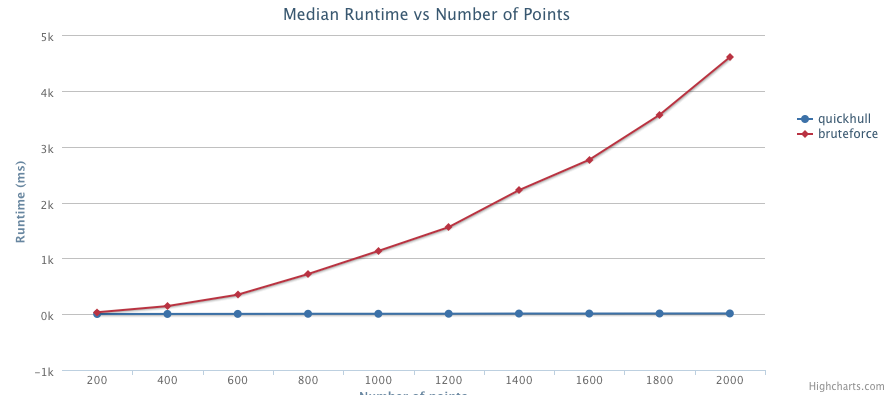
\includegraphics[scale=0.3]{qh-v-bf-cloud.png} 
\end{figure}

\begin{figure}
	\caption{Quickhull vs. brute-force on circular data}
	\centering
	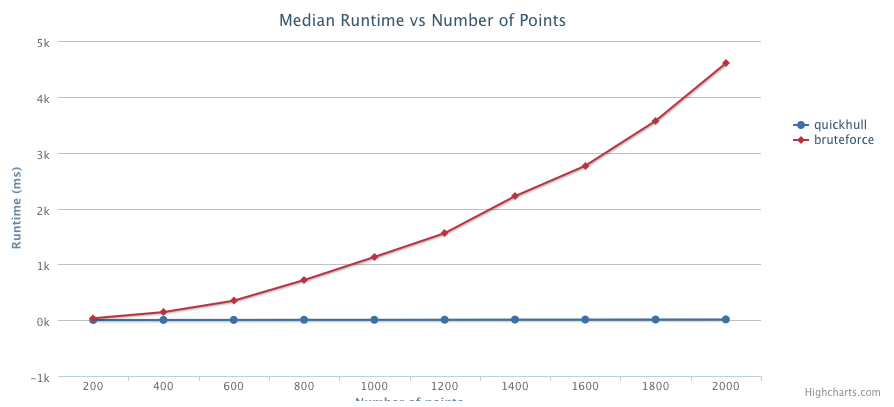
\includegraphics[scale=0.3]{qh-v-bf-circle.png} 
\end{figure}

Because the Quickhull algorithm was so much faster than the brute-force, we created a chart with Quickhull alone to illustrate its behavior:

\begin{figure}
	\caption{Quickhull scaling on point-cloud data}
	\centering
	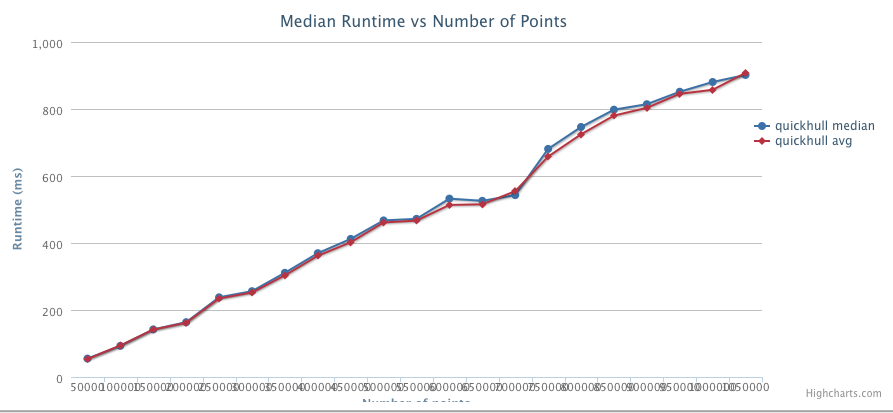
\includegraphics[scale=0.3]{qh-only.png} 
\end{figure}

Again, we were surprised because the chart shows linear, if not sub-linear, time results for the Quickhull algorithm, when the algorithm itself s $O(n log n)$. In looking into the data, we did notice that each run took longer than its predecessors, especially when the number points grew to approach 1,000,000. Our belief is that some of this data skew is due to garbage collection, but we can offer no explanation for the fact that the algorithm performance scales an entire order of magnitude lower than theoretically possible.

\subsection{Other Convex Hull Algorithms}
One popular, fast, quick hull algorithm is divide and conquer. This algorithm involves recursively dividing the points into two sets. When a base case is reached a convex hull of these subsets is calculated and then merged into neighboring point sets. As with most divide and conquer algorithms, this algorithm is easily parallelized to improve performance on modern multiprocessor systems.
Grahams scan is one of the most popular fast convex hull algorithms, with a worst case running time of $O(nlog(n))$. This algorithm first performs a clockwise sorting of the points and then determines, in order, which points are on the convex hull. Like Quickhull, this algorithm provides a substantial speed improvement over the brute force algorithm with the cost of added code complexity. Unlike Quickhull or divide and conquer, this algorithm does not easily parallelize.
\section{Summary}
When initially setting out to implement Quickhull in JavaScript, we were excited to develop a visually-rich tool for exploring this algorithm. By using modern web development techniques, we were able to rapidly create a graphical, animated implementation of the convex hull problem space. This visual representation proved extremely helpful in debugging Quickhull on large datasets.

A modern web browser is a surprisingly rich development environment, providing a REPL, debugging, and profiling tools. The quality of the individual tools varies heavily both between and within each browser. We were able to lean very heavily on the console API defined by FireBug but extended by WebKit to provide programmatic access to the script profiles, which greatly simplified data collection. However, this integrated environment does have its downsides: when we encountered issues with anomalous data, we were unable to easily verify our suspicions that garbage collection pauses were the cause.

\subsection{Further work}
Some topics came up during the development of this project which we would like to explore further:

\begin{itemize}
\item
Conducting a more detailed study of our performance results across multiple browsers and headless JavaScript environments to help explain the discrepancies we found between the expected and observed time scaling
\item
An exploration of a JavaScript arbitrary precision library to confirm our suspicions of floating-point error being the cause of the pathological cases of near-horizontal and -vertical lines
\item
Modification of the Quickhull implementation to use an explicit call tree managed by an interactive animation process to allow stepping through the animation, which could be used as an instructive aid
\end{itemize}

\nocite{Princeton:QH}
\nocite{CLRS}

\bibliographystyle{plain}
\bibliography{report}

\end{document}
